\section{CGA numerical experiments and finite-range estimates}
\label{sec:numerics}

\subsection{Model problems and error measures}

We consider the variational models of \Cref{sec:pgeometry} on \(\Omega=(0,1)^d\), with \(d=1,2\). Smooth exact solutions satisfying homogeneous natural boundary conditions are prescribed, and the corresponding loads are determined from the governing equations. \Cref{tab:cases} summarizes the model parameters and activation degrees. For the pure and regularized \(p\)-energies, the approximations satisfy the zero-mean constraint.

\begin{table}[!htbp]
\centering
\small
\caption{Model problems and parameters.}
\label{tab:cases}
\begin{tabular}{@{}lccc@{}}
\toprule
Energy & \(d\) & \(p\) & \(k\) \\
\midrule
Linear reaction--diffusion & 1 & --- & 3 \\
Cubic semilinear & 1 & --- & 3 \\
Hyperbolic-sine semilinear & 2 & --- & 3 \\
Pure \(p\)-Laplacian & 1 & 4 & 3 \\
Pure \(p\)-Laplacian & 2 & 4 & 3 \\
Regularized \(p\)-Laplacian, \(\varepsilon=0.1\) & 2 & 4 & 3 \\
Reaction \(p\)-Laplacian & 2 & 4 & 3 \\
Pure \(p\)-Laplacian & 1 & 5 & 1 \\
\bottomrule
\end{tabular}
\end{table}

For a raw \(\mathrm{ReLU}^k\) ridge function \(\varphi\), let \(P_\circ\) denote mean removal in the pure and regularized \(p\)-models and the identity otherwise. With \(Q_{\mathrm{tr}}\) denoting the quadrature used to evaluate the energy and its derivative, the computational atoms are
\[
g_Q=\frac{P_\circ\varphi}{\mathcal N_Q(P_\circ\varphi)},
\]
where
\[
\mathcal N_Q(v)=
\begin{cases}
\bigl[Q_{\mathrm{tr}}(|v|^2+|\nabla v|^2)\bigr]^{1/2},
& \text{linear and semilinear models},\\[2mm]
\bigl[Q_{\mathrm{tr}}(\sum_{i=1}^d|\partial_i v|^p)\bigr]^{1/p},
& \text{pure and regularized \(p\)-models},\\[2mm]
\bigl[Q_{\mathrm{tr}}(|v|^p+\sum_{i=1}^d|\partial_i v|^p)\bigr]^{1/p},
& \text{reaction \(p\)-model}.
\end{cases}
\]
For the \(p\)-models, the normalization and reported Sobolev errors use the componentwise gradient convention above. The energies and the natural \(V\)-map use the Euclidean gradient norm.

The finite-pool CGA constructs nested approximation spaces by selecting linearly independent atoms according to the evaluated derivative score and reoptimizing all coefficients in each enlarged space. The approximation dimension \(N\) is the number of selected independent atoms, equivalently the dimension of the current trial space. In this section, the error curves are sampled at dyadic dimensions \(N=2^j\), which are also used to compute the local convergence orders. The prescribed solutions and further implementation details are given in the supplementary material.

For the linear and semilinear cases we report the energy gap and
\[
 e_{H^1}(\widehat G_N)=\frac{\norm{\widehat G_N-u^*}_{H^1}}{\norm{u^*}_{H^1}}.
\]
For the pure and regularized \(p\)-models we report the relative gradient
seminorm, with the componentwise convention
\[
 |v|_{1,p}=\left(\int_\Omega\sum_{i=1}^d|\partial_i v|^p\dd x\right)^{1/p},
 \qquad e_{\nabla,p}(\widehat G_N)=
 \frac{|\widehat G_N-u^*|_{1,p}}{|u^*|_{1,p}}.
\]
For the reaction \(p\)-model, the reported relative error uses the full norm
\(\|v\|_{W^{1,p}}=(\|v\|_{L^p}^p+|v|_{1,p}^p)^{1/p}\).
On the zero-mean space, the gradient seminorm and full Sobolev norm are equivalent and have the same theoretical error powers. Each relative metric uses its own denominator. The relative natural distance is \(e_V(\widehat G_N)=d_{V,\bullet}(\widehat G_N,u^*)/d_{V,\bullet}(0,u^*)\), with a nonzero denominator for the benchmark profiles. For evaluation quadrature \(Q_{\rm ev}\), write
\[
 \widehat\delta_{N,Q_{\rm ev}}=\E_{Q_{\rm ev}}(\widehat G_N)-\E_{Q_{\rm ev}}(u^*),
\]
where \(\E_{Q_{\rm ev}}\) denotes the quadrature-evaluated energy. The numerical records retain signed energy differences, and energy summaries use the metric-valid observations defined in \Cref{sec:results}.
The dyadic local order is
\[
 \operatorname{ord}_N(e)=\log_2\!\left(\frac{e(N/2)}{e(N)}\right).
\]
The figures and tables report energy gaps, relative Sobolev errors, and relative natural distances, together with the corresponding dyadic local orders.

\subsection{Reference powers and metric conversion}

For \(\relu^k\) atoms, the Hilbert-space approximation exponent associated with the smooth-ridge
entropy estimate is
\[
 \beta_H=\frac12+\frac{2(k-1)+1}{2d}.
\]
The dashed segments show the reference powers \(N^{-2\beta_H}\) for the energy gap, \(N^{-\beta_H}\) for the \(H^1\) error or natural \(V\)-distance, and \(N^{-2\beta_H/p}\) for the Sobolev error of a standard \(p\)-structure energy. These powers follow the conversion in \Cref{cor:metric-rates}. Their exponents are prescribed, and the vertical offsets are set by the median log error over the last up to three positive dyadic states.

\subsection{Linear and cubic calibration}

\Cref{fig:cga-linear-cubic} shows the retained dyadic states for the linear and cubic multifrequency
problems.  Both curves decrease rapidly after about 32 atoms.  Between \(N=128\) and 256, the
linear energy and \(H^1\) orders are 6.083 and 3.042, whereas the cubic orders are 6.896 and 3.448; the
corresponding terminal relative \(H^1\) errors are \(1.247\times10^{-4}\) and
\(1.215\times10^{-4}\).

\begin{figure}[!htbp]
\centering
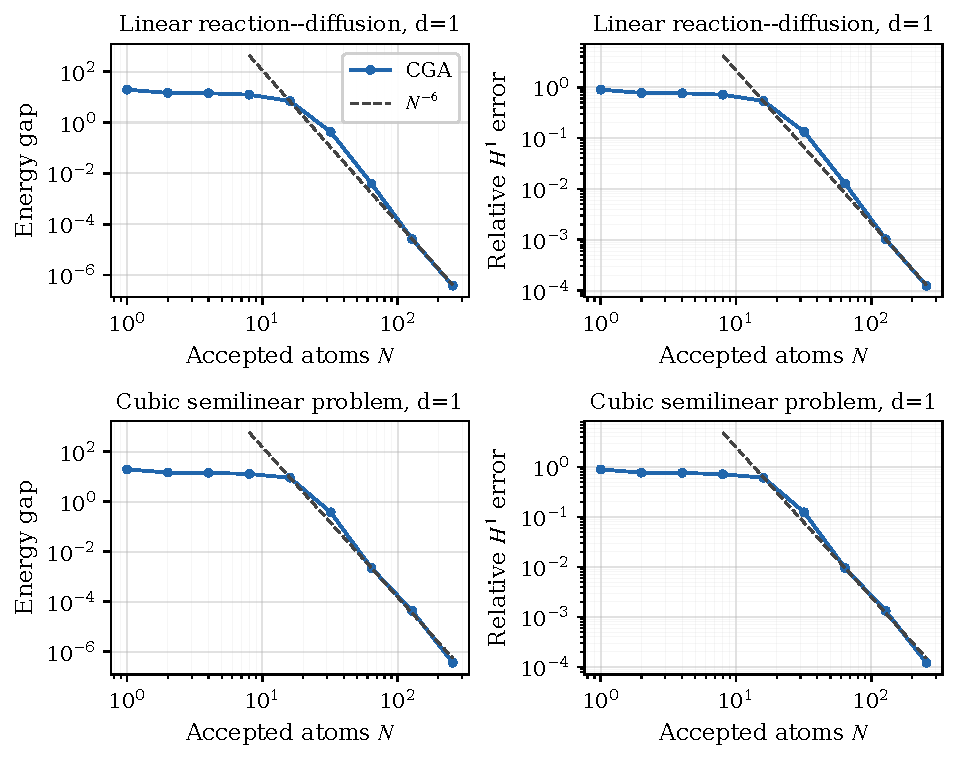
\includegraphics[width=0.96\textwidth]{cga_linear_cubic.pdf}
\caption{CGA errors at dyadic retained widths for the linear and cubic problems. The dashed segments show the reference powers \(N^{-6}\) for the energy gap and \(N^{-3}\) for the relative \(H^1\) error.}
\label{fig:cga-linear-cubic}
\end{figure}

For the two-dimensional sinh model, the relative \(H^1\) error decreases from \(4.074\times10^{-3}\) at \(N=256\) to \(1.990\times10^{-3}\) at \(N=512\). The local orders are 1.793 on \(128\to256\) and 1.034 on \(256\to512\); the trajectory is shown in the supplementary figures.
\FloatBarrier

\subsection{Numerical results for the pure and regularized \texorpdfstring{\(p=4\)}{p=4} models}

\Cref{fig:cga-p4-representative} reports the energy gap, relative gradient \(L^4\) seminorm error, and relative \(V\)-distance for the one- and two-dimensional pure \(p=4\) models. At \(N=128\), the one-dimensional case has relative gradient and \(V\)-errors of \(1.579\times10^{-5}\) and \(1.680\times10^{-6}\). For the two-dimensional case, the energy and \(V\)-orders on \(128\to256\) are 3.410 and 1.703. From \(N=256\) to 512, the \(V\)-distance decreases, while the relative gradient errors are \(2.494\times10^{-3}\) and \(3.601\times10^{-3}\), respectively.

\begin{figure}[!htbp]
\centering
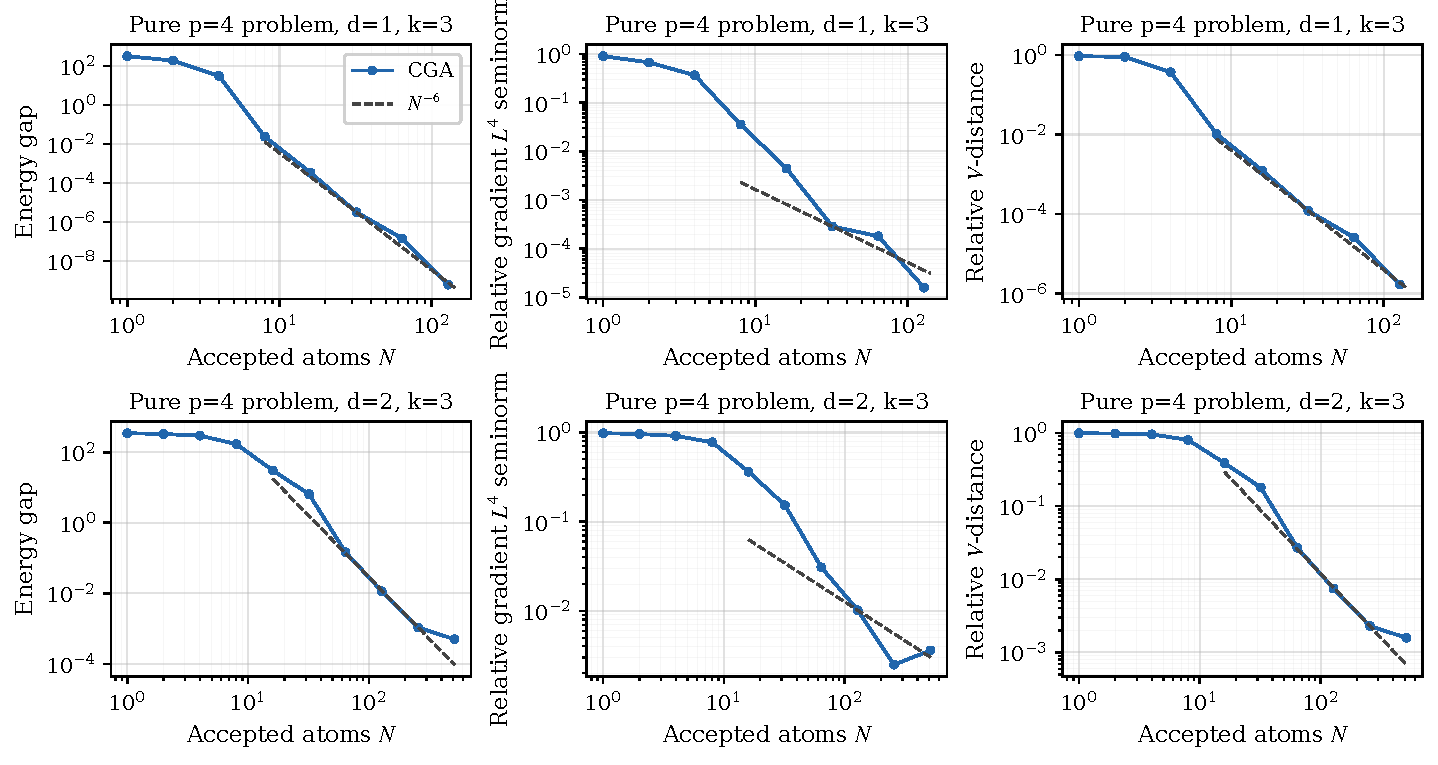
\includegraphics[width=0.98\textwidth]{cga_p4_representative.pdf}
\caption{CGA errors at dyadic retained widths for the pure \(p=4\) models. Columns show the energy gap, relative gradient \(L^4\) seminorm error, and relative \(V\)-distance. Dashed segments show powers \(N^{-6},N^{-3/2},N^{-3}\) in one dimension and \(N^{-7/2},N^{-7/8},N^{-7/4}\) in two dimensions, in column order.}
\label{fig:cga-p4-representative}
\end{figure}

The dyadic values for the semilinear and $p=4$ cases are supplied in the supplementary numerical records. The regularized and reaction trajectories show the same separation between the natural-distance and Sobolev metrics as the representative pure cases.

\FloatBarrier

\subsection{Finite-trajectory error estimates for quartic energies}
\label{sec:finite-trajectory-numerics}
\label{sec:fractional-innovation-p4}

We apply the projection estimates and quartic energy comparison of \Cref{sec:c5-source} to the one-dimensional pure and regularized \(p=4\) models. We take activation degree \(k=3\), exact solution \(u^*(x)=\cos(2\pi x)\), and \(\varepsilon=0\) and \(0.1\), respectively. The approximate source representation is constructed at \(N=8\) and then held fixed. The comparison constants are determined on the states \(N=8,\ldots,32\), while the decrease constant is determined from the corresponding transitions \(N\to N+1\), \(N=8,\ldots,31\). Each trajectory is then continued to \(N=64\), with the source representation and these constants unchanged.

The approximate-source estimate bounds the squared projection error \(r_N^2\), and the quartic comparison transfers this estimate to the energy error of the computed states. Throughout the calibration range, the resulting energy bounds cover the computed energy errors for both models.

To examine the power-type decrease condition, we prescribe the benchmark exponent \(\alpha_{\mathrm{bench}}=6\) and define
\[
U_j=
\left(
r_8^{-2/\alpha_{\mathrm{bench}}}
+\frac{c_0j}{\alpha_{\mathrm{bench}}}
\right)^{-\alpha_{\mathrm{bench}}},
\qquad 1\le j\le24.
\]
Under the stepwise decrease condition
\[
\gamma_N^2\ge
c_0r_N^{\,2+2/\alpha_{\mathrm{bench}}},
\]
the finite-range estimate in \Cref{thm:c5-power} gives \(r_{8+j}^2\le U_j\). Applying \Cref{cor:c5-power-metrics} yields energy, natural-distance, and \(W^{1,4}\)-error bounds proportional to \(U_j\), \(U_j^{1/2}\), and \(U_j^{1/4}\), respectively.

During continuation, the same decrease condition is tested with the calibrated value of \(c_0\). Among the 32 transitions \(N\to N+1\), \(N=32,\ldots,63\), the condition holds for 27 transitions in the pure model and 28 in the regularized model. The source quantities, comparison constants, and quadrature consistency checks are provided in the supplementary material.

